\section{Biểu diễn Ảnh và Video Kỹ thuật số}
\label{sec:digital_image_and_video_representation}

\subsection{Giới thiệu: Từ Thế giới Tương tự đến Mạng lưới Pixel}
\label{subsec:analog_to_digital_intro}

Thế giới thị giác mà chúng ta cảm nhận là một dòng chảy liên tục của ánh sáng, màu sắc và hình dạng. Tuy nhiên, một máy tính chỉ có thể làm việc với các giá trị rời rạc, hữu hạn. Quá trình biến đổi một cảnh vật lý liên tục thành một đối tượng mà máy tính có thể lưu trữ và xử lý là một trong những kỳ công nền tảng của kỹ thuật số. Nó bao gồm hai bước cốt lõi: \textbf{lấy mẫu (sampling)} để rời rạc hóa không gian, và \textbf{lượng tử hóa (quantization)} để rời rạc hóa cường độ.

Trong phần này, chúng ta sẽ mổ xẻ cấu trúc của một hình ảnh và video kỹ thuật số ở mức độ chi tiết nhất. Chúng ta sẽ bắt đầu bằng cách mô hình hóa hình ảnh như một hàm toán học, sau đó đi sâu vào quá trình rời rạc hóa để tạo ra lưới pixel quen thuộc. Tiếp theo, chúng ta sẽ khám phá một chủ đề cực kỳ quan trọng trong Thị giác Máy tính: các không gian màu. Tại sao một ảnh RGB là không đủ? Tại sao việc tách biệt độ sáng và màu sắc lại là một ý tưởng mang tính cách mạng cho cả thuật toán thị giác và nén dữ liệu? Cuối cùng, chúng ta sẽ mở rộng các khái niệm này sang miền thời gian để hiểu cách một video, về bản chất là một chuỗi các khung hình, được mã hóa và nén một cách hiệu quả để có thể truyền tải qua mạng internet.

Hiểu rõ cách dữ liệu thị giác được cấu trúc và biểu diễn là bước đầu tiên không thể thiếu để xây dựng bất kỳ hệ thống Thị giác Máy tính nào. Nó quyết định cách chúng ta đọc, xử lý và thiết kế các thuật toán hoạt động trên dữ liệu đó.

\subsection{Mô hình hóa Ảnh Kỹ thuật số: Một Góc nhìn Toán học}
\label{subsec:digital_image_modeling}

Trước khi trở thành một tệp tin trên máy tính, một hình ảnh có thể được mô tả một cách hình thức như một hàm số.

\subsubsection{Ảnh như một Hàm số Liên tục}
\label{subsubsec:image_as_function}
Một hình ảnh lý tưởng có thể được xem như một hàm số 2 chiều, $I(x, y)$, trong đó:
\begin{itemize}
    \item $(x, y)$ là các tọa độ không gian liên tục trên một mặt phẳng hình chữ nhật, ví dụ $x \in [0, W], y \in [0, H]$.
    \item $I(x, y)$ là giá trị cường độ sáng (intensity) tại tọa độ đó. Đối với ảnh xám, $I(x, y)$ là một giá trị vô hướng.
\end{itemize}
Đối với ảnh màu, hàm này trả về một vector các giá trị, mỗi giá trị tương ứng với một kênh màu. Ví dụ, trong mô hình RGB, hàm ảnh là $\mathbf{I}(x, y) = [R(x, y), G(x, y), B(x, y)]^T$, trong đó mỗi hàm thành phần biểu diễn cường độ của kênh màu đỏ, lục, và lam.

Mô hình hàm số này rất hữu ích về mặt lý thuyết, nhưng nó không thể được xử lý trực tiếp bởi máy tính. Chúng ta cần rời rạc hóa nó.

\subsubsection{Quá trình Rời rạc hóa: Lấy mẫu và Lượng tử hóa}
\label{subsubsec:discretization}
Quá trình chuyển đổi từ hàm ảnh liên tục $I(x, y)$ sang một ảnh kỹ thuật số bao gồm hai bước chính:

\begin{description}
    \item[Lấy mẫu (Sampling):] Đây là quá trình rời rạc hóa các tọa độ không gian $(x, y)$. Chúng ta áp một lưới hình chữ nhật lên hàm ảnh liên tục và chỉ lấy giá trị của hàm tại các giao điểm của lưới. Mỗi giao điểm này trở thành một \textbf{pixel} (picture element). Kết quả của quá trình lấy mẫu là một ma trận các giá trị cường độ.
    
    \begin{center}
        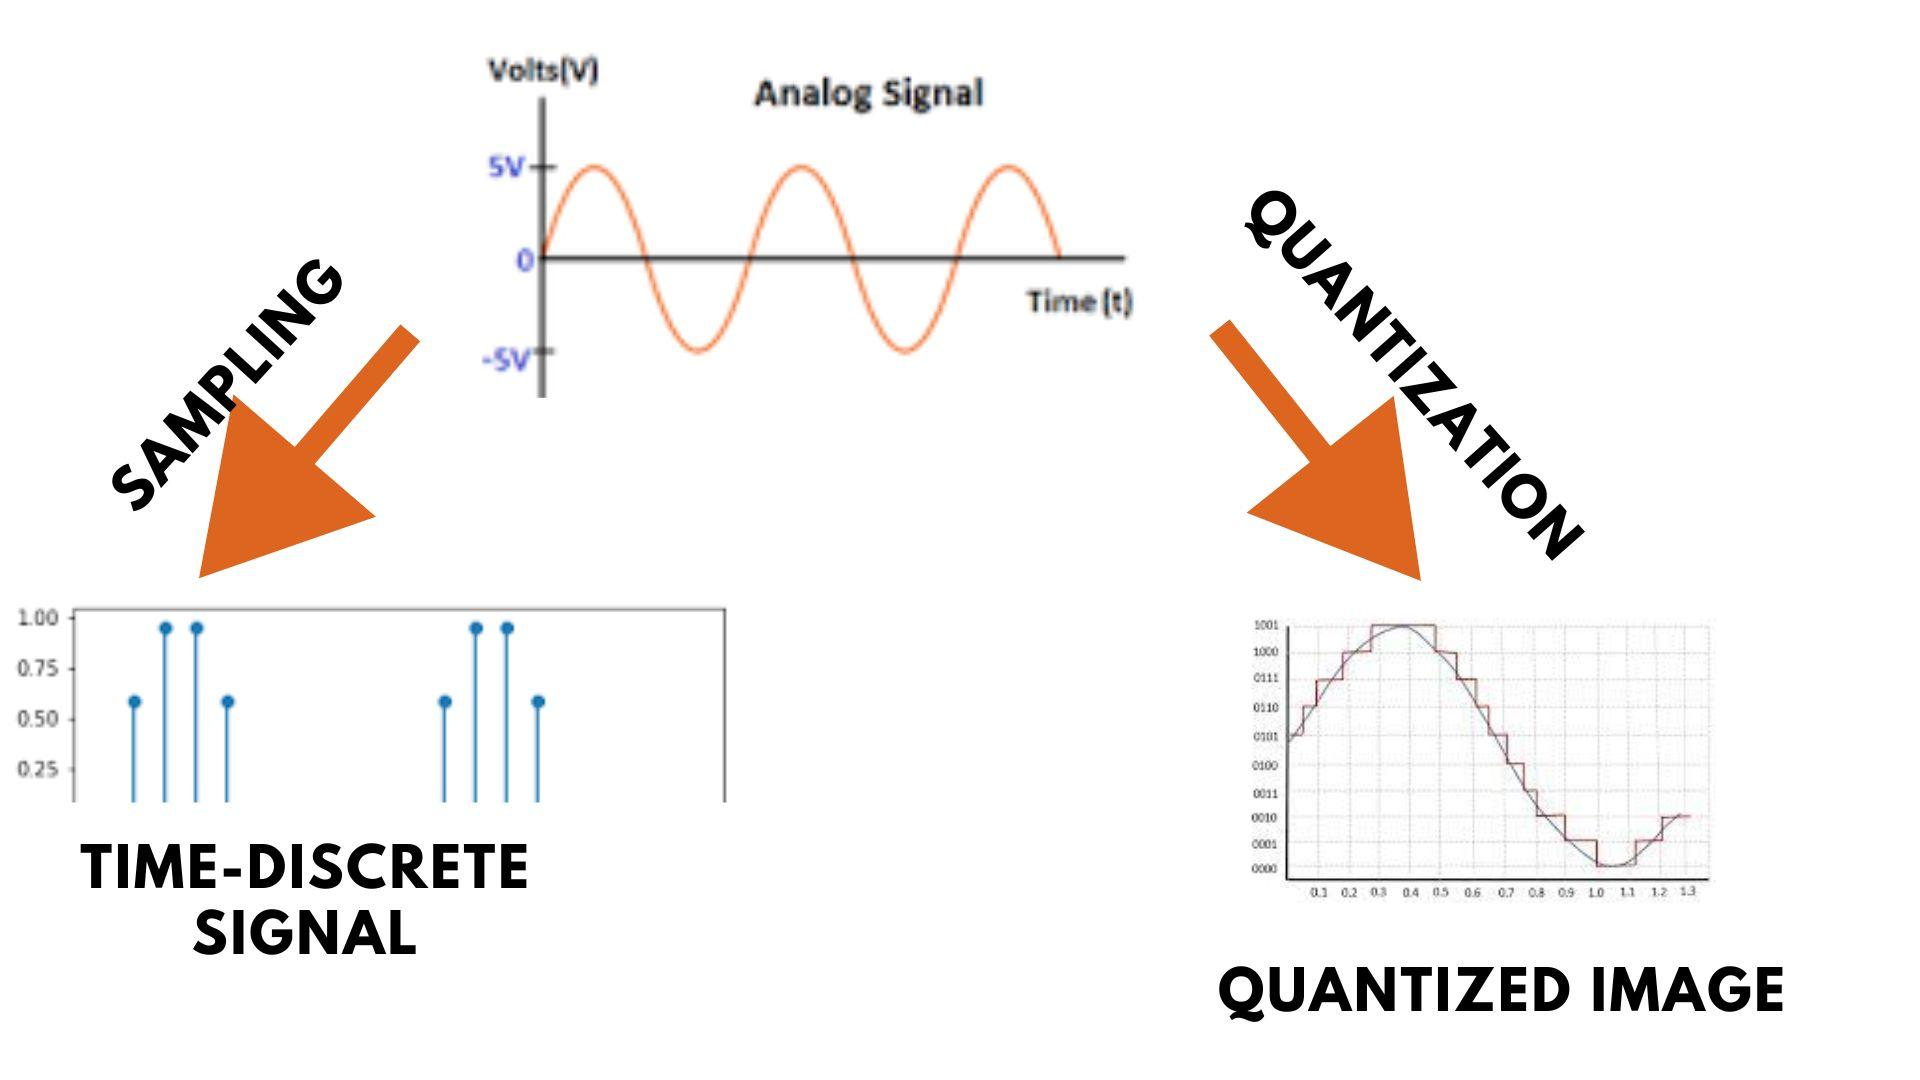
\includegraphics[width=0.8\textwidth]{images/sampling_and_quantization.jpg}
        \captionof{figure}{Minh họa quá trình lấy mẫu và lượng tử hóa. (Trái) Lấy mẫu rời rạc hóa tín hiệu theo trục không gian. (Giữa) Hàm cường độ sáng liên tục của một tín hiệu 1D. (Phải) Lượng tử hóa rời rạc hóa giá trị cường độ tại mỗi mẫu thành các mức hữu hạn.}
        \label{fig:sampling_quantization}
    \end{center}
    
    Chất lượng của quá trình lấy mẫu phụ thuộc vào "mật độ" của lưới. Mật độ này được gọi là \textbf{độ phân giải (resolution)} của ảnh, thường được biểu thị bằng số lượng pixel theo chiều rộng và chiều cao (ví dụ: $1920 \times 1080$). Theo \textbf{Định lý Lấy mẫu Nyquist-Shannon}, để tái tạo lại một tín hiệu một cách hoàn hảo, tần số lấy mẫu phải lớn hơn ít nhất hai lần tần số cao nhất có trong tín hiệu. Nếu không, sẽ xảy ra hiện tượng \textbf{aliasing}, trong đó các tần số cao bị "nhầm lẫn" thành các tần số thấp, gây ra các hoa văn giả (ví dụ: Moiré pattern).
    
    \item[Lượng tử hóa (Quantization):] Sau khi lấy mẫu, giá trị cường độ tại mỗi pixel vẫn có thể là một số thực liên tục. Lượng tử hóa là quá trình rời rạc hóa các giá trị cường độ này thành một tập hợp các mức hữu hạn. Số lượng mức được quyết định bởi \textbf{độ sâu bit (bit depth)} của ảnh.
    \begin{itemize}
        \item Một ảnh 8-bit, là loại phổ biến nhất, sử dụng 8 bit để biểu diễn cường độ của mỗi kênh màu tại mỗi pixel. Điều này cho phép có $2^8 = 256$ mức cường độ, thường là từ 0 (đen) đến 255 (trắng).
        \item Một ảnh 1-bit chỉ có $2^1 = 2$ mức, thường là 0 và 1, tạo ra một ảnh nhị phân (đen và trắng).
    \end{itemize}
    Lượng tử hóa với ít mức hơn sẽ gây ra hiện tượng \textbf{posterization}, trong đó các dải màu chuyển tiếp mượt mà bị thay thế bằng các vùng màu sắc nét, tạo ra các "dải" hoặc "viền" giả trong ảnh.
\end{description}

Sau hai quá trình này, một ảnh xám $H \times W$ với độ sâu 8-bit trở thành một ma trận số nguyên $\mathbf{I} \in \mathbb{Z}^{H \times W}$, trong đó mỗi phần tử $I_{ij} \in \{0, 1, \dots, 255\}$.

\subsection{Các Không gian Màu (Color Spaces): Hơn cả RGB}
\label{subsec:color_spaces}

Mắt người không cảm nhận màu sắc theo các kênh Đỏ, Lục, Lam một cách độc lập. Các không gian màu khác nhau được phát triển để mô hình hóa màu sắc theo những cách phù hợp hơn cho các ứng dụng cụ thể, từ hiển thị, in ấn, cho đến các thuật toán Thị giác Máy tính.

\subsubsection{RGB: Mô hình Cộng cho Hiển thị}
\label{subsubsec:rgb_colorspace}
Không gian màu RGB (Red, Green, Blue) là một mô hình màu cộng, có nghĩa là các màu sắc được tạo ra bằng cách cộng ánh sáng từ ba nguồn màu gốc.
\begin{itemize}
    \item \textbf{Nguồn gốc:} Dựa trên cách hoạt động của các màn hình (ví dụ: CRT, LCD, LED), trong đó mỗi pixel được tạo thành từ ba điốt phát quang phụ (sub-pixel) màu đỏ, lục, và lam.
    \item \textbf{Biểu diễn:} Một màu được biểu diễn bởi một bộ ba $(R, G, B)$. Khi $R=G=B=0$, ta có màu đen. Khi $R=G=B=255$ (trong hệ 8-bit), ta có màu trắng.
    \item \textbf{Hạn chế trong CV:} RGB không có tính \textbf{đồng nhất về mặt tri giác (perceptually uniform)}. Điều này có nghĩa là một khoảng cách Euclid nhất định trong không gian RGB không tương ứng với một sự khác biệt về màu sắc cảm nhận được như nhau. Ví dụ, sự khác biệt giữa $(0, 255, 0)$ và $(0, 245, 0)$ (hai sắc thái của màu lục) được cảm nhận khác hoàn toàn so với sự khác biệt giữa $(128, 128, 0)$ và $(118, 128, 0)$. Hơn nữa, thông tin về cường độ sáng và màu sắc bị trộn lẫn với nhau. Một sự thay đổi nhỏ về ánh sáng trong môi trường sẽ làm thay đổi cả ba giá trị R, G, B, gây khó khăn cho các thuật toán cần sự ổn định về màu sắc.
\end{itemize}

\begin{center}
    
\includegraphics[width=0.8\textwidth]{color_spaces.jpg}
    \captionof{figure}{Minh họa hai không gian màu phổ biến. (Trái) Mô hình khối lập phương RGB, một mô hình cộng phù hợp cho các thiết bị hiển thị. (Phải) Mô hình hình trụ HSV, tách biệt Màu sắc (Hue), Độ bão hòa (Saturation) và Độ sáng (Value), gần với cách con người cảm nhận màu sắc hơn.}
    \label{fig:color_spaces}
\end{center}

\subsubsection{Grayscale (Ảnh xám): Tách biệt Cường độ sáng}
\label{subsubsec:grayscale}
Chuyển đổi ảnh màu sang ảnh xám là một bước tiền xử lý phổ biến để giảm độ phức tạp của bài toán. Tuy nhiên, việc chuyển đổi này không đơn giản là lấy trung bình các kênh RGB. Nó tính đến độ nhạy khác nhau của mắt người đối với các màu sắc khác nhau. Công thức chuẩn (theo ITU-R BT.601) là:
\begin{equation}
    Y' = 0.299 \times R + 0.587 \times G + 0.114 \times B
    \label{eq:grayscale_conversion}
\end{equation}
\textbf{Trực giác:} Các hệ số trong công thức phản ánh việc mắt người nhạy cảm nhất với màu lục ($0.587$), tiếp theo là màu đỏ ($0.299$), và ít nhạy cảm nhất với màu lam ($0.114$). Điều này đảm bảo rằng độ sáng cảm nhận được của ảnh xám sẽ gần với ảnh màu gốc nhất.

\subsubsection{HSV: Mô hình Trực quan của Con người}
\label{subsubsec:hsv_colorspace}
Không gian màu HSV (Hue, Saturation, Value) sắp xếp lại hình học của RGB để phù hợp hơn với cách con người mô tả màu sắc.
\begin{itemize}
    \item \textbf{Hue (Tông màu):} Đại diện cho "loại" màu sắc thuần túy (đỏ, vàng, lục, lam,...). Nó được biểu diễn như một góc trên một vòng tròn màu, từ 0 đến 360 độ.
    \item \textbf{Saturation (Độ bão hòa):} Đại diện cho "độ thuần khiết" của màu. Saturation bằng 0 có nghĩa là màu xám, trong khi Saturation cao có nghĩa là màu sắc rực rỡ.
    \item \textbf{Value (Giá trị sáng):} Đại diện cho độ sáng hoặc tối của màu.
\end{itemize}
\textbf{Ưu điểm trong CV:} Sự tách biệt giữa tông màu (H) và độ sáng (V) là cực kỳ hữu ích. Ví dụ, trong bài toán theo dõi một vật thể màu đỏ, chúng ta có thể định nghĩa một khoảng giá trị cho kênh H (ví dụ, H gần 0 độ hoặc 360 độ) và cho phép các kênh S và V thay đổi trong một khoảng rộng. Điều này làm cho thuật toán trở nên \textbf{bất biến với sự thay đổi ánh sáng (illumination invariant)}.

\subsubsection{Y'CbCr: Ngôn ngữ của Nén Video}
\label{subsubsec:ycbcr_colorspace}
Không gian màu Y'CbCr là nền tảng của hầu hết các chuẩn nén ảnh (JPEG) và video (MPEG, H.264). Giống như HSV, nó cũng tách biệt thông tin độ sáng và màu sắc, nhưng theo một cách khác:
\begin{itemize}
    \item \textbf{Y':} Kênh Luma, biểu diễn độ sáng (tương tự như ảnh xám).
    \item \textbf{Cb, Cr:} Hai kênh Chroma, biểu diễn sự khác biệt về màu sắc (Cb: blue-difference, Cr: red-difference).
\end{itemize}
\textbf{Lý do tồn tại:} Hệ thống thị giác của con người nhạy cảm với sự thay đổi về độ sáng hơn nhiều so với sự thay đổi về màu sắc. Kỹ thuật \textbf{Chroma Subsampling (Lấy mẫu phụ Tín hiệu màu)} tận dụng đặc điểm này. Thay vì lưu trữ thông tin Cb, Cr cho mỗi pixel, chúng ta có thể lưu trữ chúng với độ phân giải thấp hơn.
\begin{description}
    \item[4:4:4:] Không nén. Mỗi pixel có giá trị Y', Cb, Cr riêng.
    \item[4:2:2:] Cb và Cr được lấy mẫu với một nửa độ phân giải theo chiều ngang. Một cặp pixel kề nhau theo chiều ngang sẽ chia sẻ chung một giá trị Cb và Cr.
    \item[4:2:0:] Đây là dạng phổ biến nhất cho video tiêu dùng. Cb và Cr được lấy mẫu với một nửa độ phân giải ở cả chiều ngang và chiều dọc. Một khối 4 pixel ($2 \times 2$) sẽ chia sẻ chung một giá trị Cb và Cr. Điều này giúp giảm một nửa băng thông cần thiết cho thông tin màu sắc mà mắt người gần như không nhận ra sự khác biệt.
\end{description}

\subsection{Biểu diễn Video Kỹ thuật số: Tận dụng Sự Dư thừa Thời gian}
\label{subsec:digital_video_representation}

Một video có thể được xem như một chuỗi các hình ảnh (khung hình - frames) được chiếu liên tiếp. Tuy nhiên, việc lưu trữ video dưới dạng một loạt các tệp ảnh JPEG độc lập là cực kỳ không hiệu quả.

\subsubsection{Dư thừa Không gian và Thời gian}
Nén video hiệu quả dựa trên việc khai thác hai loại dư thừa:
\begin{itemize}
    \item \textbf{Dư thừa Không gian (Spatial Redundancy):} Sự tương quan giữa các pixel trong cùng một khung hình. Về cơ bản, đây chính là loại dư thừa mà nén ảnh như JPEG giải quyết.
    \item \textbf{Dư thừa Thời gian (Temporal Redundancy):} Sự tương quan giữa các khung hình liên tiếp. Trong hầu hết các video, phần lớn nội dung của cảnh không thay đổi hoặc chỉ di chuyển một chút từ khung hình này sang khung hình tiếp theo. Đây là "mỏ vàng" cho việc nén video.
\end{itemize}

\subsubsection{Dự đoán Liên khung (Inter-frame Prediction)}
Các chuẩn nén video hiện đại như H.264/AVC và H.265/HEVC sử dụng một cấu trúc gọi là \textbf{Nhóm các Hình ảnh (Group of Pictures - GOP)} để khai thác sự dư thừa thời gian. Một GOP thường bao gồm ba loại khung hình:

\begin{description}
    \item[I-frames (Intra-coded frames):] Đây là các khung hình "khóa". Chúng được nén độc lập, giống như một ảnh JPEG, mà không cần tham chiếu đến bất kỳ khung hình nào khác. Một GOP luôn bắt đầu bằng một I-frame. Chúng tốn nhiều dung lượng nhất nhưng cho phép bắt đầu giải mã từ vị trí đó.
    \item[P-frames (Predicted frames):] Các khung hình này được mã hóa bằng cách chỉ lưu trữ sự khác biệt so với một khung hình I-frame hoặc P-frame trước đó. Sự khác biệt này được mã hóa bằng các \textbf{vector chuyển động (motion vectors)}, mô tả cách các khối pixel đã di chuyển. Chúng tiết kiệm dung lượng hơn nhiều so với I-frames.
    \item[B-frames (Bi-directionally predicted frames):] Đây là loại khung hình hiệu quả nhất. Chúng được mã hóa bằng cách tham chiếu đến cả các khung hình trong quá khứ và tương lai. Điều này cho phép chúng xử lý các trường hợp như một đối tượng bị che khuất tạm thời.
\end{description}

\begin{center}
    
\includegraphics[width=1.0\textwidth]{gop_structure.png}
    \captionof{figure}{Minh họa cấu trúc một Nhóm các Hình ảnh (GOP) đơn giản trong nén video. I-frame là khung hình đầy đủ. P-frames dự đoán chuyển động từ các khung hình trước đó. B-frames dự đoán từ cả quá khứ và tương lai, mang lại hiệu quả nén cao nhất. Các mũi tên chỉ ra sự phụ thuộc trong quá trình mã hóa/giải mã.}
    \label{fig:gop_structure}
\end{center}

\subsubsection{Codec và Container}
Hai khái niệm thường bị nhầm lẫn:
\begin{itemize}
    \item \textbf{Codec (Coder-Decoder):} Là thuật toán hoặc tiêu chuẩn dùng để nén và giải nén dữ liệu video (ví dụ: H.264, H.265/HEVC, AV1). Nó định nghĩa cách các I, P, B-frames được tạo ra.
    \item \textbf{Container (Định dạng chứa):} Là định dạng tệp tin bao bọc xung quanh các dòng dữ liệu video và âm thanh đã được nén, cùng với siêu dữ liệu (metadata) và thông tin đồng bộ hóa (ví dụ: MP4, MKV, AVI). Một tệp MP4 có thể chứa video được nén bằng H.264 hoặc H.265.
\end{itemize}

\subsection{Biểu diễn trong Bộ nhớ và Lập trình}
\label{subsec:memory_representation}
Khi một ảnh được tải vào bộ nhớ để xử lý bằng các thư viện như OpenCV hoặc Pillow, nó thường được chuyển đổi thành một mảng đa chiều của NumPy.
\begin{minted}[fontsize=\footnotesize, frame=single, linenos=true]{python}
import cv2
import numpy as np

# Load an image from disk
# cv2.imread loads the image in BGR format by default
image_bgr = cv2.imread('my_cat.jpg')

# Check the data type and shape
print(f"Data type: {image_bgr.dtype}") # Typically uint8
print(f"Shape: {image_bgr.shape}") # e.g., (480, 640, 3) -> (Height, Width, Channels)

# Access a single pixel at row 100, column 50
# Note the (row, col) or (y, x) indexing
pixel_value = image_bgr[100, 50]
print(f"Pixel at (100, 50): {pixel_value}") # e.g., [158 168 180] (B, G, R)

# Convert to RGB for use with libraries like Matplotlib
image_rgb = cv2.cvtColor(image_bgr, cv2.COLOR_BGR2RGB)

# Convert to Grayscale
image_gray = cv2.cvtColor(image_bgr, cv2.COLOR_BGR2GRAY)
print(f"Grayscale shape: {image_gray.shape}") # e.g., (480, 640)

# Normalize pixel values to the [0, 1] range for deep learning models
# This is a crucial preprocessing step
image_normalized = image_bgr.astype(np.float32) / 255.0
print(f"Normalized data type: {image_normalized.dtype}") # float32
print(f"Min/Max values: {np.min(image_normalized)}, {np.max(image_normalized)}")
\end{minted}
Như đoạn mã trên minh họa, một ảnh màu được biểu diễn như một tensor bậc 3 (H, W, C). Các kênh màu thường là 3 (BGR trong OpenCV). Việc hiểu rõ cấu trúc này, thứ tự các chiều, và kiểu dữ liệu là cực kỳ quan trọng để thực hiện các thao tác xử lý ảnh một cách chính xác.

\section*{Tài liệu tham khảo}
\begin{itemize}
    \item[1] Gonzalez, R. C.; Woods, R. E. \textit{Digital Image Processing}. 4th ed. Pearson, 2018. (Đây là cuốn sách giáo khoa kinh điển về xử lý ảnh, giải thích rất chi tiết về lấy mẫu, lượng tử hóa và không gian màu).
    \item[2] Poynton, C. \textit{A Technical Introduction to Digital Video}. Wiley, 1996.
    \item[3] Richardson, I. E. G. \textit{The H.264 Advanced Video Compression Standard}. 2nd ed. Wiley, 2010.
    \item[4] Szeliski, R. \textit{Computer Vision: Algorithms and Applications}. 2nd ed. Springer, 2022. (Chương 2 cung cấp một tổng quan xuất sắc về biểu diễn ảnh).
    \item[5] Donoho, D. L. Compressed Sensing. \textit{IEEE Transactions on Information Theory} \textbf{2006}, \textit{52}(4), 1289–1306.
    \item[6] Candès, E. J.; Romberg, J.; Tao, T. Robust uncertainty principles: Exact signal reconstruction from highly incomplete frequency information. \textit{IEEE Transactions on Information Theory} \textbf{2006}, \textit{52}(2), 489-509.
    \item[7] Kingma, D. P.; Ba, J. Adam: A Method for Stochastic Optimization. In \textit{Proceedings of the 3rd International Conference on Learning Representations (ICLR)}, 2015.
\end{itemize}